\documentclass[a4paper, landscape]{article}

\usepackage{graphicx} % Allows including images
\usepackage{stackengine}
\usepackage{scalerel}
\usepackage{xcolor}
\usepackage{geometry}
\usepackage{multicol}
\usepackage{listings}

\graphicspath{{./../img/}}
\renewcommand{\abstractname}{}
\renewcommand{\tt}[1]{\texttt{#1}}

\newcommand\dangersign[1][2ex]{%
  \renewcommand\stacktype{L}%
  \scaleto{\stackon[1.3pt]{\color{red}$\triangle$}{\tiny !}}{#1}%
}

\newcommand{\warn}[1]{\begin{center}
\begin{tabular}{ c  p{12cm} }
\dangersign[22pt] & \vspace{-0.6cm} #1
\end{tabular}
\end{center}}

\geometry{
 a4paper,
 left=30mm,
 right=30mm,
 top=30mm,
 bottom=30mm
 }

\lstset{language=Python,
		commentstyle=\color{gray},
		keywordstyle=\color{blue},
		numberstyle=\color{yellow},
		stringstyle=\color{purple}
}

\renewcommand{\tt}[1]{\textcolor{blue}{\texttt{#1}}}
\newcommand{\grey}[1]{\textcolor{purple}{\it{(#1)}}}
\geometry{left=.1cm,
			right=.1cm,
			top=.3cm,
			bottom=.3cm}

\title{theia Quick Reference}

\begin{document}
\begin{center}
\large \tt{theia} Quick Reference (version 0.1.3)
\end{center}

\fontsize{9}{9}

\begin{tabular}{| p{.4cm} | p{15cm}| p{3cm} | p{8.4cm} |}
\hline
\textbf{Key} & \textbf{Input Order and defaults} & \textbf{Action on beams} \grey{Increase of strayness for R~on~HR, T~on~HR, R~on~AR, T~on~AR}& \textbf{Remarks} \\ \hline \hline
\tt{bo} & \tt{X}, \tt{Y}, \tt{Z}~=~0 \grey{origin of bench} & & This will shift all the coordinates of the following optics and beams (until the next \tt{bo} line) by the amounts given here (blank \tt{bo} line to return to general system).\\ \hline

\tt{bm} &  \tt{Wx}~=~1.mm, \tt{Wy}~=~1.mm \grey{waist sizes}, \tt{WDistx}~=~0., \tt{WDisty}~=~0. \grey{waist positions from beam origin}, \tt{Wl}~=~1064.nm, \tt{P}~=~1.W, \tt{X}~=~0., \tt{Y}~=~0., \tt{Z}~=~0. \grey{position of origin in space}, \tt{Theta}~=~pi/2., \tt{Phi}~=~0. \grey{orientation} , \tt{Alpha}~=~0. \grey{rotation of eigenbase for orthogonal beams}, \tt{Ref}~=~None & &\tt{Alpha = 0.} $\leftrightarrow$ eigen X is $\perp$ to beam direction and has maximum $Z$ component. If direction is $\pm e_Z$ then eigen X is $\pm e_X$\\ \hline

\tt{mr} &   \tt{X}~=~0., \tt{Y}~=~0., \tt{Z}~=~0. \grey{position of center of HR chord}, \tt{Theta}~=~pi/2., \tt{Phi}~=~0. \grey{orientation of HR Norm, pointing out}, \tt{Wedge}~=~0., \tt{Alpha}~=~0. \grey{wedge and wedge rotation}, \tt{HRK}~=~0.01, \tt{ARK}~=~0. \grey{curvatures}, \tt{Diameter}~=~10.cm \grey{of the construction cylinder}, \tt{Thickness}~=~2.cm, \tt{N}~=~1.4585, \tt{HRr}~=~.99, \tt{HRt}~=~.01, \tt{ARr}~=~.1, \tt{ARt}~=~.9 \grey{power reflectances and transmittances}, \tt{KeepI}~=~False, \tt{Ref}~=~None & 0, +1, +1, 0 & Wedges are counted positive if you \textit{add} material when you increase the wedge.\\ \hline

\tt{bs} &   \tt{X}~=~0., \tt{Y}~=~0., \tt{Z}~=~0. \grey{position of center of HR chord}, \tt{Theta}~=~pi/2., \tt{Phi}~=~0. \grey{orientation of HR Norm, pointing out}, \tt{Wedge}~=~0., \tt{Alpha}~=~0. \grey{wedge and wedge rotation}, \tt{HRK}~=~0., \tt{ARK}~=~0. \grey{curvatures}, \tt{Diameter}~=~10.cm \grey{of the construction cylinder}, \tt{Thickness}~=~2.cm, \tt{N}~=~1.4585, \tt{HRr}~=~.5, \tt{HRt}~=~.5, \tt{ARr}~=~.1, \tt{ARt}~=~.9 \grey{power reflectances and transmittances}, \tt{KeepI}~=~False, \tt{Ref}~=~None & 0, 0, 0, 0 & This is very similar to mirror \tt{bm}, but has different default values and never increases the strayness of beams.\\ \hline


\tt{th} &   \tt{X}~=~0., \tt{Y}~=~0., \tt{Z}~=~0. \grey{position of center of lens}, \tt{Theta}~=~pi/2., \tt{Phi}~=~0. \grey{orientation of HR Norm, pointing out}, \tt{Focal}~=~10.cm,  \tt{Diameter}~=~5.cm, \tt{R}~=~.1, \tt{T}~=~.9 \grey{power reflectance and transmittance, per surface}, \tt{KeepI}~=~False,  \tt{Ref}~=~False & +1, 0, 0, +1 & All parameters which are not present here are internally adjusted in order to fit the input \tt{Focal}, \tt{Diameter} and a \tt{N}~=~1.4584 value for the optical index\\ \hline

\tt{tk} &  \tt{X}~=~0., \tt{Y}~=~0., \tt{Z}~=~0. \grey{position of apex of HR face of lens}, \tt{Theta}~=~pi/2., \tt{Phi}~=~0. \grey{orientation of HR Norm, pointing out}, \tt{K1}~=~.01, \tt{K2}~=~.001 \grey{curvatures}, \tt{Diameter}~=~5.cm,  \tt{Thickness}~=~2.cm, \tt{N}~=~1.4585, \tt{R}~=~.1, \tt{T}~=~.9 \grey{power reflectance and transmittance}, \tt{KeepI}~=~False,  \tt{Ref}~=~None & +1, 0, 0, +1 &\tt{Thickness}: on optical axis (from apex to apex). Note that in this case the provided HR center corresponds to the position of the \it{apex} of the HR surface, on the contrary of mirrors. \\ \hline

\tt{sp} &   \tt{RonHR}~=~0, \tt{TonHR}~=~0, \tt{RonAR}~=~0, \tt{TonAR}~=~0 \grey{actions on beams}, \tt{X}~=~0., \tt{Y}~=~0., \tt{Z}~=~0. \grey{position of center of HR chord}, \tt{Theta}~=~pi/2., \tt{Phi}~=~0. \grey{orientation of HR Norm, pointing out}, \tt{Wedge}~=~0., \tt{Alpha}~=~0. \grey{wedge and wedge rotation}, \tt{HRK}~=~0.01, \tt{ARK}~=~0. \grey{curvatures}, \tt{Diameter}~=~10.cm, \tt{Thickness}~=~2.cm, \tt{N}~=~1.4585, \tt{HRr}~=~.99, \tt{HRt}~=~.01, \tt{ARr}~=~.1, \tt{ARt}~=~.9 \grey{power reflectances and transmittances}, \tt{KeepI}~=~False, \tt{Ref}~=~None & User defined by \tt{RonHR}, \tt{TonHR}, \tt{RonAR}, \tt{TonAR} & This is the object which allows you to specify exactly the action of each surface on reflected and transmitted beams.\\ \hline


\tt{bd} &  \tt{X}~=~0., \tt{Y}~=~0., \tt{Z}~=~0. \grey{position of center of HR}, \tt{Theta}~=~pi/2., \tt{Phi}~=~0. \grey{orientation of HR Norm, pointing out}, \tt{Diameter}~=~5.cm,  \tt{Thickness}~=~2.cm,  \tt{Ref}~=~None & Stops all beams & \\ \hline

\tt{gh} &   \tt{X}~=~0., \tt{Y}~=~0., \tt{Z}~=~0. \grey{position of center of HR}, \tt{Theta}~=~pi/2., \tt{Phi}~=~0. \grey{orientation of HR Norm, pointing out}, \tt{Diameter}~=~5.cm, \tt{Ref}~=~None & Transmits beams without modification, no reflected beam &This component does not affect the beams, but just allows to have a new entry in the output file for the beam emerging from the ghost surface. It does not have a 3D rendering object associated. \\ \hline
\end{tabular}

\begin{multicols}{3}
\paragraph{Keys.} \tt{bo} (new coordinate origin), \tt{bm} (input beam), \tt{mr} (mirror), \tt{bs} (beam splitter), \tt{th} (thin lens), \tt{tk} (thick lens), \tt{sp} (special surface), \tt{bd} (beam dump), \tt{gh} (ghost surface)
\paragraph{Units.}(km, m = 1., cm, mm, um, nm), (kW, W = 1., mW, uW, nW), (THz, GHz, MHz, kHz, Hz = 1., mHz, uHz), (ppm = 1.e-6, rad = 1., deg), pi
\paragraph{Functions.} sin, cos, tan, arcsin, arccos, arctan, sqrt, exp


\paragraph{Notes.}\begin{itemize}
\item \tt{Theta}, \tt{Phi} are spherical coordinates around $e_Z$ and \tt{Phi = 0.} $\leftrightarrow~ + e_X$
\item All constructors can be called without arguments, all parameters have default values.
\end{itemize}

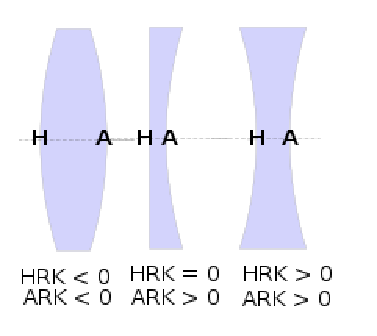
\includegraphics[scale=.6]{convention.pdf}
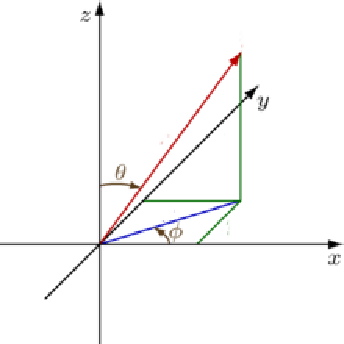
\includegraphics[scale=.6]{spherical.pdf}

\end{multicols}
\end{document}
